\documentclass[11pt,a4paper]{article}
\usepackage{../templates/igcsephysics}

\begin{document}

\frontpage

\newpage
\setcounter{question}{0}

\question{Fig. \figref{fig:electric-bicycle} shows an electrically powered bicycle.}{8}
\examfigure{fig:electric-bicycle}{%
  \includegraphics[
    page=2,
    trim=35mm 185mm 35mm 26mm,
    clip,
    width=120mm
  ]{../0625_s22_qp_42.pdf}%
}

\qtext{The battery can deliver a power of 600 W for 60 min.}

\partsubquestion{a}{i}{Calculate the energy, in joules, stored in the battery when fully charged.}
\working[26mm]
\answer{energy}{J}{3}

\subpartquestion{ii}{State the form of energy stored by the battery.}
\subpartwrittenanswer{ }{1}

\partquestion{b}{The bicycle has a motor with an electrical input power of 250 W.}
\parttext{Calculate the time for which the battery can power the bicycle.}
\working[26mm]
\answer{time}{s}{2}

\partquestion{c}{State two environmental benefits of using an electrically powered bicycle instead of a small motorcycle.}
\twowrittenlines
\marksright{2}
\totalmarks

\newpage

\question{Fig. \figref{fig:pulley-bench} shows two objects connected by a cord passing over a pulley.}{9}
\examfigure{fig:pulley-bench}{%
  \includegraphics[
    page=3,
    trim=48mm 211mm 43mm 36mm,
    clip,
    width=95mm
  ]{../0625_s22_qp_42.pdf}%
}

\qtext{The 2.0 kg object is released from rest and accelerates at 4.0 m/s\textsuperscript{2}.}

\partquestion{a}{Calculate the resultant force acting on the 2.0 kg object.}
\working[25mm]
\answer{force}{N}{2}

\partquestion{b}{Calculate the upward force exerted by the cord on the 3.0 kg object.}
\working[28mm]
\answer{force}{N}{3}

\partsubquestion{c}{i}{The objects have a constant acceleration.}
\subparttext{Show that the speed of the objects 0.80 s after release is 3.2 m/s.}
\working[24mm]
\marksright{2}

\subpartquestion{ii}{A card of width 2.0 cm passes through a beam of light at this speed. Calculate the time taken for the card to pass through the beam.}
\working[25mm]
\answer{time}{s}{2}
\totalmarks

\newpage

\questionpart{a}{Fig. \figref{fig:river-canoe} shows water in a river moving parallel to the river bank at 4.0m/s and a canoe travelling in the river.}{8}
\examfigure{fig:river-canoe}{%
  \includegraphics[
    page=4,
    trim=25mm 181mm 25mm 31mm,
    clip,
    width=135mm
  ]{../0625_s22_qp_42.pdf}%
}

\parttext{The canoe travels at 2.5m/s relative to the water and heads at an angle of 38\textdegree{} to the river bank.}

\parttext{Draw a scale diagram to determine the canoe's resultant velocity and state the scale you used.}
\working[70mm]
\rightanswerline[80mm]{scale}
\rightanswerline[80mm]{magnitude of resultant velocity}
\rightanswerline[80mm]{direction of resultant velocity (angle from the river bank)}
\rightanswermark{4}

\partquestion{b}{Explain why the resultant velocity is not in the same direction as the canoe points.}
\writtenline{ }
\writtenline{ }
\marksright{2}
\totalmarks

\newpage

\question{A student investigates the resistance of a wire.}{10}
\figplaceholder[fig:resistance-wire]{11}{4.2}

\partquestion{a}{Complete the table headings for the measurements needed in this experiment.}

\begin{center}
\renewcommand{\arraystretch}{1.8}
\begin{tabular}{|p{38mm}|p{38mm}|p{38mm}|}
\hline
\textbf{Length of wire / cm} & & \\ \hline
20 & & \\ \hline
40 & & \\ \hline
60 & & \\ \hline
80 & & \\ \hline
\end{tabular}
\end{center}
\marksright{2}

\partquestion{b}{Describe how the student can use the measurements to determine the resistance of the wire.}
\answerbox[34mm]
\marksright{4}

\partquestion{c}{State two precautions that improve the reliability of the results.}
\twowrittenlines
\marksright{2}

\partquestion{d}{On the grid, sketch the expected shape of a graph of resistance against length for a uniform wire.}
\begin{center}
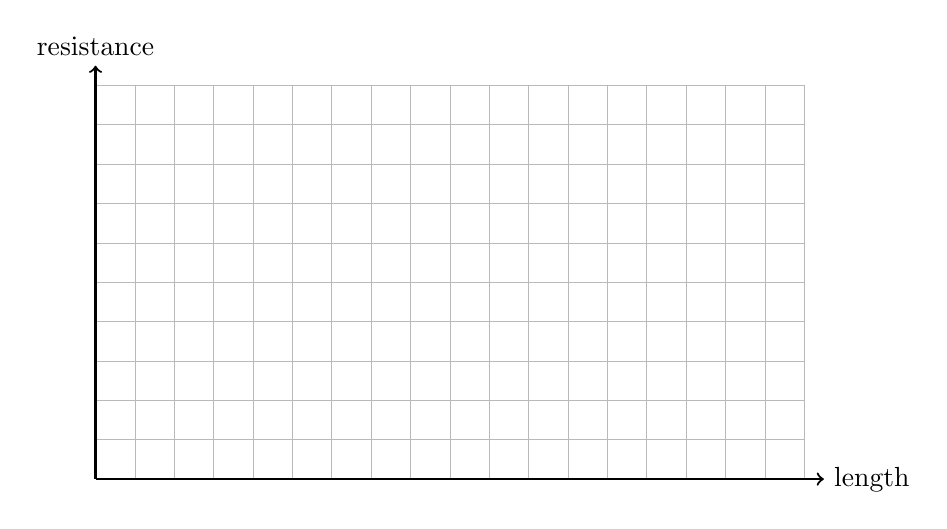
\begin{tikzpicture}[x=0.5cm,y=0.5cm]
  \draw[step=0.5cm,gray!55,very thin] (0,0) grid (18,10);
  \draw[thick,->] (0,0) -- (18.5,0) node[right] {length};
  \draw[thick,->] (0,0) -- (0,10.5) node[above] {resistance};
\end{tikzpicture}
\end{center}
\marksright{2}
\totalmarks

\blankpage

\question{This page shows the structure for adding another long question. Replace this text with your own question stem.}{6}
\partquestion{a}{Write the first part of the question here.}
\working[18mm]
\answer{answer}{unit}{2}
\partquestion{b}{Write the second part of the question here.}
\answerbox[30mm]
\marksright{4}
\totalmarks

\end{document}
